\chapter{Theory behind quantum driving}
\label{chap:physicalIntro}
This chapter heavily depends on the mathematical formalism developed in Chapter \ref{chap:mathIntro} and basic knowledge of quantum mechanics is required.

Most parts of this chapter are inspired by \citet{kolodrubez} and original notes by \citet{berry1984}, \citet{berry1989}, \citet{berry2009} with attempt to give them more rigorous meaning in the language of differential geometry. We will see, that the structure of the space of states on which the driving will occur is quite complicated. The reason is its fiber structure, where every fiber is another fiber bundle. Luckily what we will be using later on are sections of this space, which will be much easier Riemannian manifolds. 

From now on we will use natural units, so $\hbar=1$.




\section{Space of all states}
Assume parameter $\llambda\in\mathcal{U}\subset\R^d$ for $\mathcal U$ open set. This parameter controls some finite-dimensional Hamiltonian $\HH(\llambda)$, which is bounded from below and has discrete spectrum. From this we can construct the fiber bundle, such that at every point of the base manifold $\llambda\in \mathcal{U}$, we construct fiber spanning all possible states of $\H(\llambda)$, thus the fiber structure can be according to Def. \ref{def:fiberBundle} written as
$$\left(\H_{full}\coloneqq \bigcup_{\llambda\in\mathcal U} \H(\llambda),\;\;\mathcal{U}\subset \R^d,\;\;\pi,\;\; \H(\llambda) \coloneqq \bigcup_{states}\ket{\psi(\llambda)}  \right).$$
The projection is defined as $\pi(\llambda): \ket{\psi(\llambda)}\mapsto \llambda$ and $\H(\llambda)$ is Hilbert space for all pure states of $\H(\llambda)$. 
Note that some states in the $\H_{full}$ space are physically identical. Geometric intuition is displayed in fig. \ref{fig:wholeBundle}.
\begin{figure}[h]
    \centering
    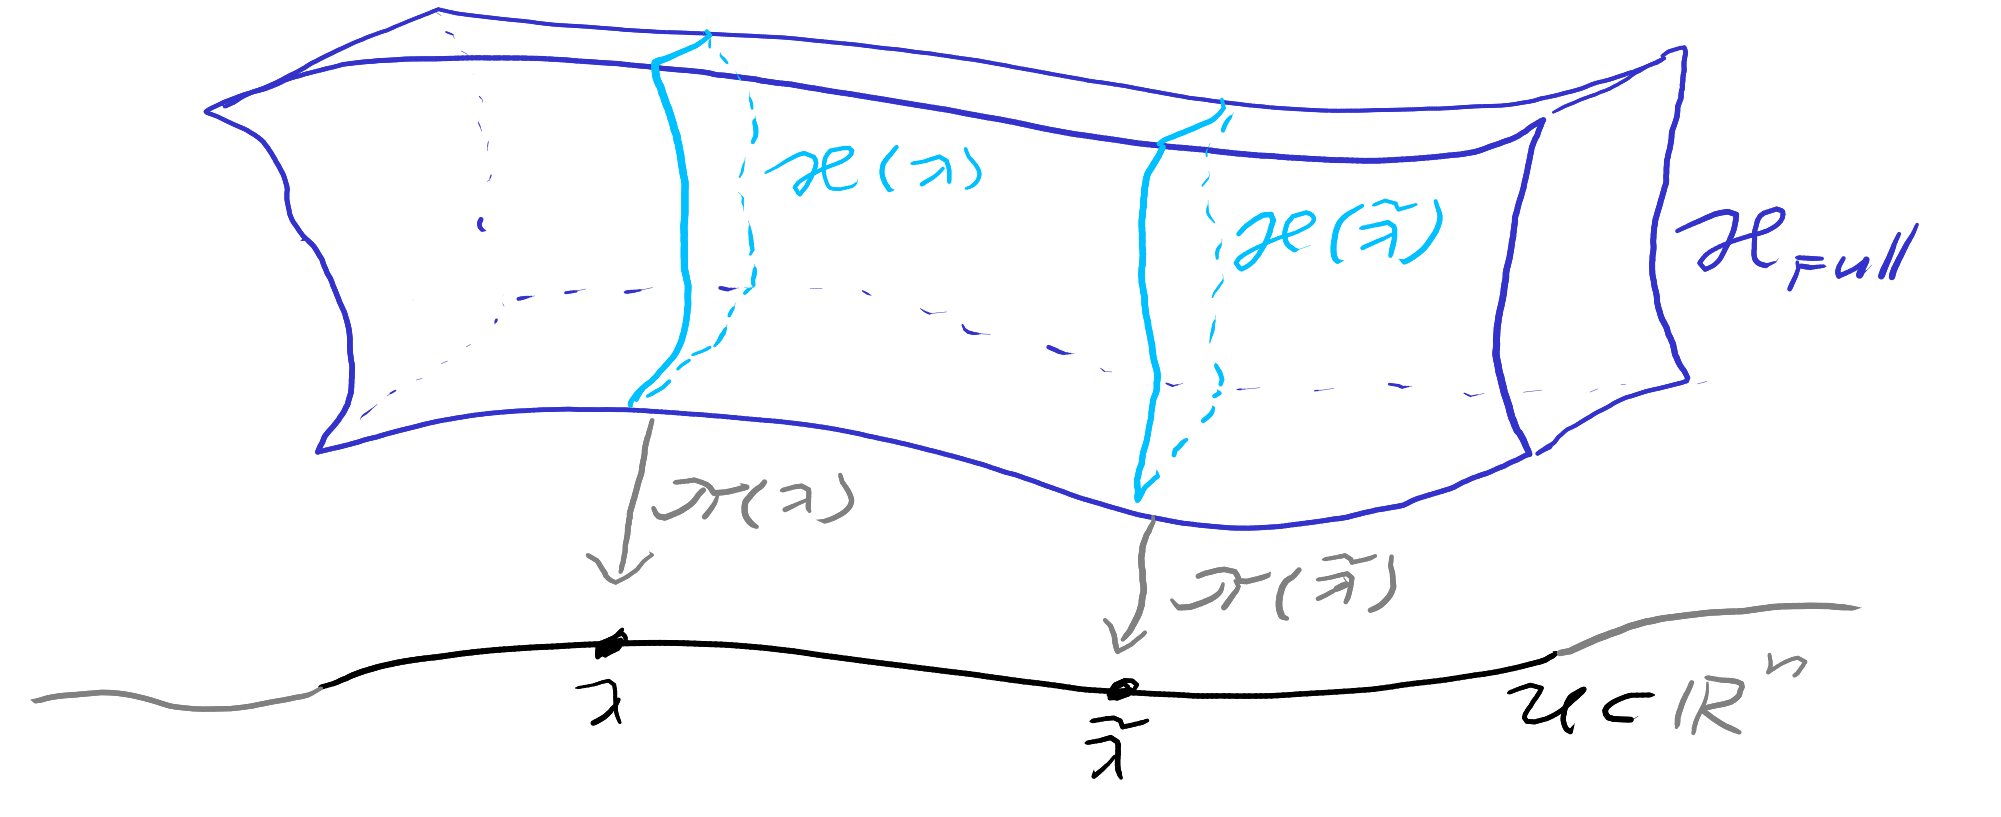
\includegraphics[width=\textwidth]{../img/manifold_basic_1.png}
\caption{Base manifold $\mathcal U\subset \R^d$ is visualized as a line. From every point $\llambda$ there is constructed one Hilbert space $\H(\llambda)$ as a fiber. The union of all these fibers is full Hilbert space $\H_{full}$.}
    \label{fig:wholeBundle}
\end{figure}






\section{Rays and bare states}
In quantum mechanics, physical observables are related to the \emph{space of rays}, defined as $\P\H\coloneqq \H/U(1)$, where elements of $U(1)$ are unitary transformations $e^{i\varphi}$ for $\varphi\in\R$. This defines the gauge symmetry between quantum states. The phase $\varphi$ is chosen the same for every vector and can be chosen arbitrarily. We cannot alter the phase of individual vectors. The geometrical intuition is drawn for any $\llambda$ on fig. \ref{fig:projectiveHilbertSpace}.
\begin{figure}[H]
    \centering
    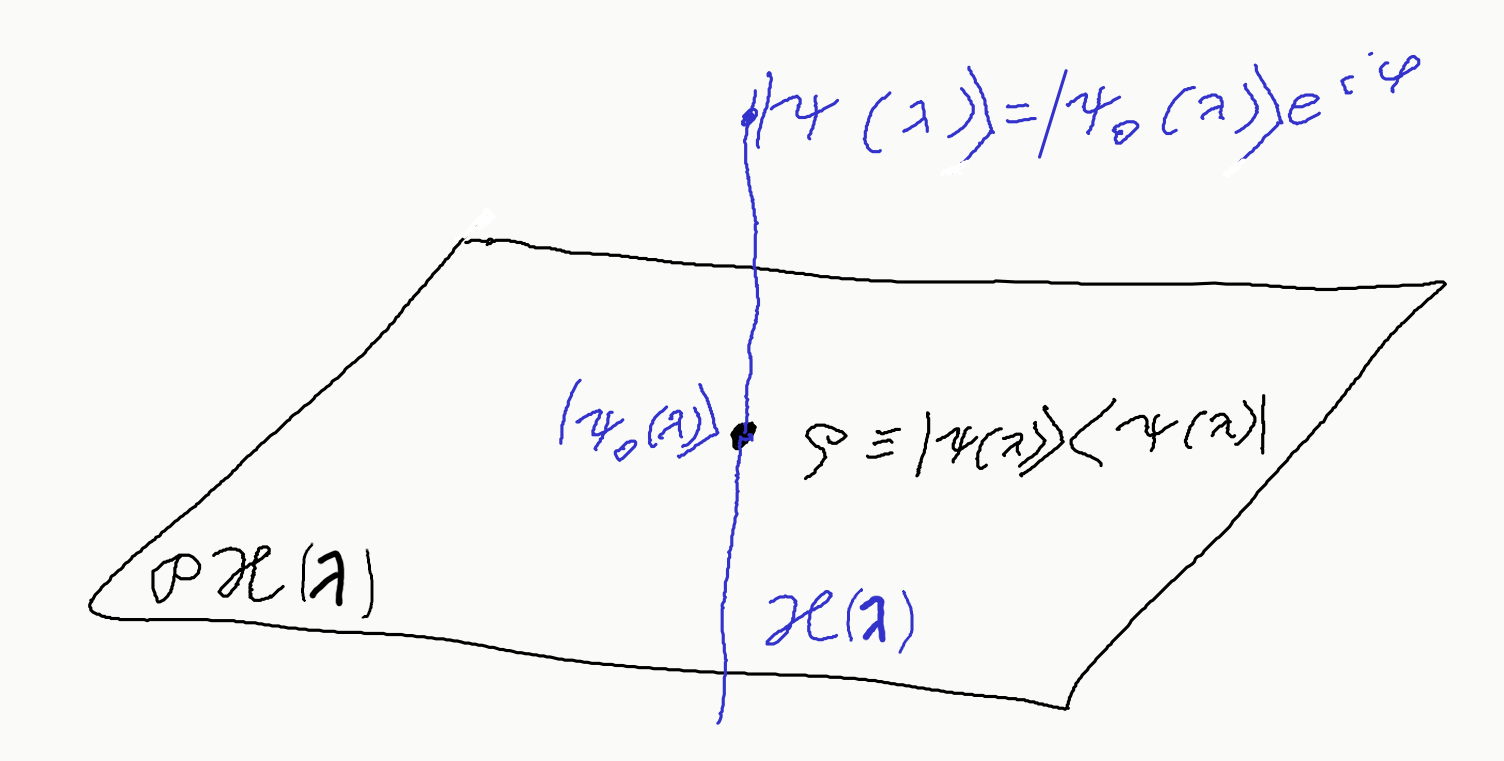
\includegraphics[width=0.8\textwidth]{../img/projectiveHilbertSpace.png}
\caption{For every $\llambda$ we have the Hilbert space $\H(\llambda)$ containing all states $e^{i\varphi}\ket{\psi(\llambda)}$. Choosing the phase $\varphi$ fixes some projective Hilbert space $\P\H$.}
    \label{fig:projectiveHilbertSpace}
\end{figure}

This resembles the fiber structure
$$\left(\H,\;\P\H,\;\pi_{rays},\;\{e^{i\varphi}| \varphi\in\R\}\right),$$
where $\pi_{rays}$ is just rule setting phase $\varphi$ to arbitrary value, which we will fix to $\varphi=0$.







\section{Sectioning the space}
Assume one begins with the state $\ket{\psi_0}$. The state then evolves along some path $\gamma\coloneqq\{\llambda(t)|t\in(0,T)\}\subset \mathcal U$ parametrized by time, for which the \Schrodinger equation
\begin{equation}
    i\hbar \der{}{t}\kpsilt = \HH(\llambda)\kpsilt
    \label{eq:schrodinger}
\end{equation}
holds. For eigenstates of instantaneous Hamiltonian it reads as energy \Schrodinger equation
\begin{equation}
    \HH(\llambda)\ket{s(\llambda)}=E_s(\llambda)\ket{s(\llambda)}.
    \label{eq:energySchrodinger}
\end{equation}
Notice that these states are independent on the trajectory $\gamma_t$.
For every $\HH(\llambda)$ its energies can be sorted from the lowest, defining the set $\sigma(\HH(\llambda))\coloneqq\{E_0,\dots,E_n\}$, which will be called \emph{spectrum of the Hamiltonian}. In this set, degeneracies are not unified into one element, therefore every $\sigma(\llambda)$ has $n$ elements. From this there exists an isomorphism between all $\sigma$-sets, and we can define \emph{section} 
$$\mathrm{sec}_s: \ket{s(\llambda)}\mapsto \mathcal{U}\subset \R^d, \quad \text{for } s\in\{0,\dots, n-1\}.$$
This maps eigenstates corresponding to energy $E_s$ to the base manifold. This mapping is similar to previously introduced $\pi$, except it chooses one point from the infinite dimensional Hilbert space and maps it to the base manifold. From this the $\sec_s$ is a isomorphism. 

Now we have constructed $n$ sections of the full Hilbert space, which are isomorphic to the base manifold. Because $\mathcal U$ is a Riemannian manifold, these so-called \emph{projective energy manifolds} $\P\M_s$, must be also Riemannian.
Special importance of the \emph{projective ground state manifold} $\P\M_0$, which will be used later on for adiabatic transports of ground states. Geometrical intuition is drawn on fig. \ref{fig:fullStructure}. 

The reason for calling these manifolds \emph{projective} is the gauge symmetry of the Schr\"odinger equation. We can change the phase of vector $\kpsi\mapsto e^{i\varphi}\kpsi$ by any $\varphi$. Unifying over all phases, we get \emph{energy manifolds}
\begin{equation}
    \M_s\coloneqq \left\{\bigcup_{\varphi\in\R} \bigcup_{\llambda\in\mathcal U} e^{i\varphi}\ket{\psi(\llambda)}\right\}
\end{equation}

Because these manifolds were created by sectioning, they are considered to be vector spaces in a geometrical sense. This was expected, because they contain quantum states, which themselves are vectors. \red{Elaborate here, construction of basis should be enough.}

\begin{figure}[H]
    \centering
    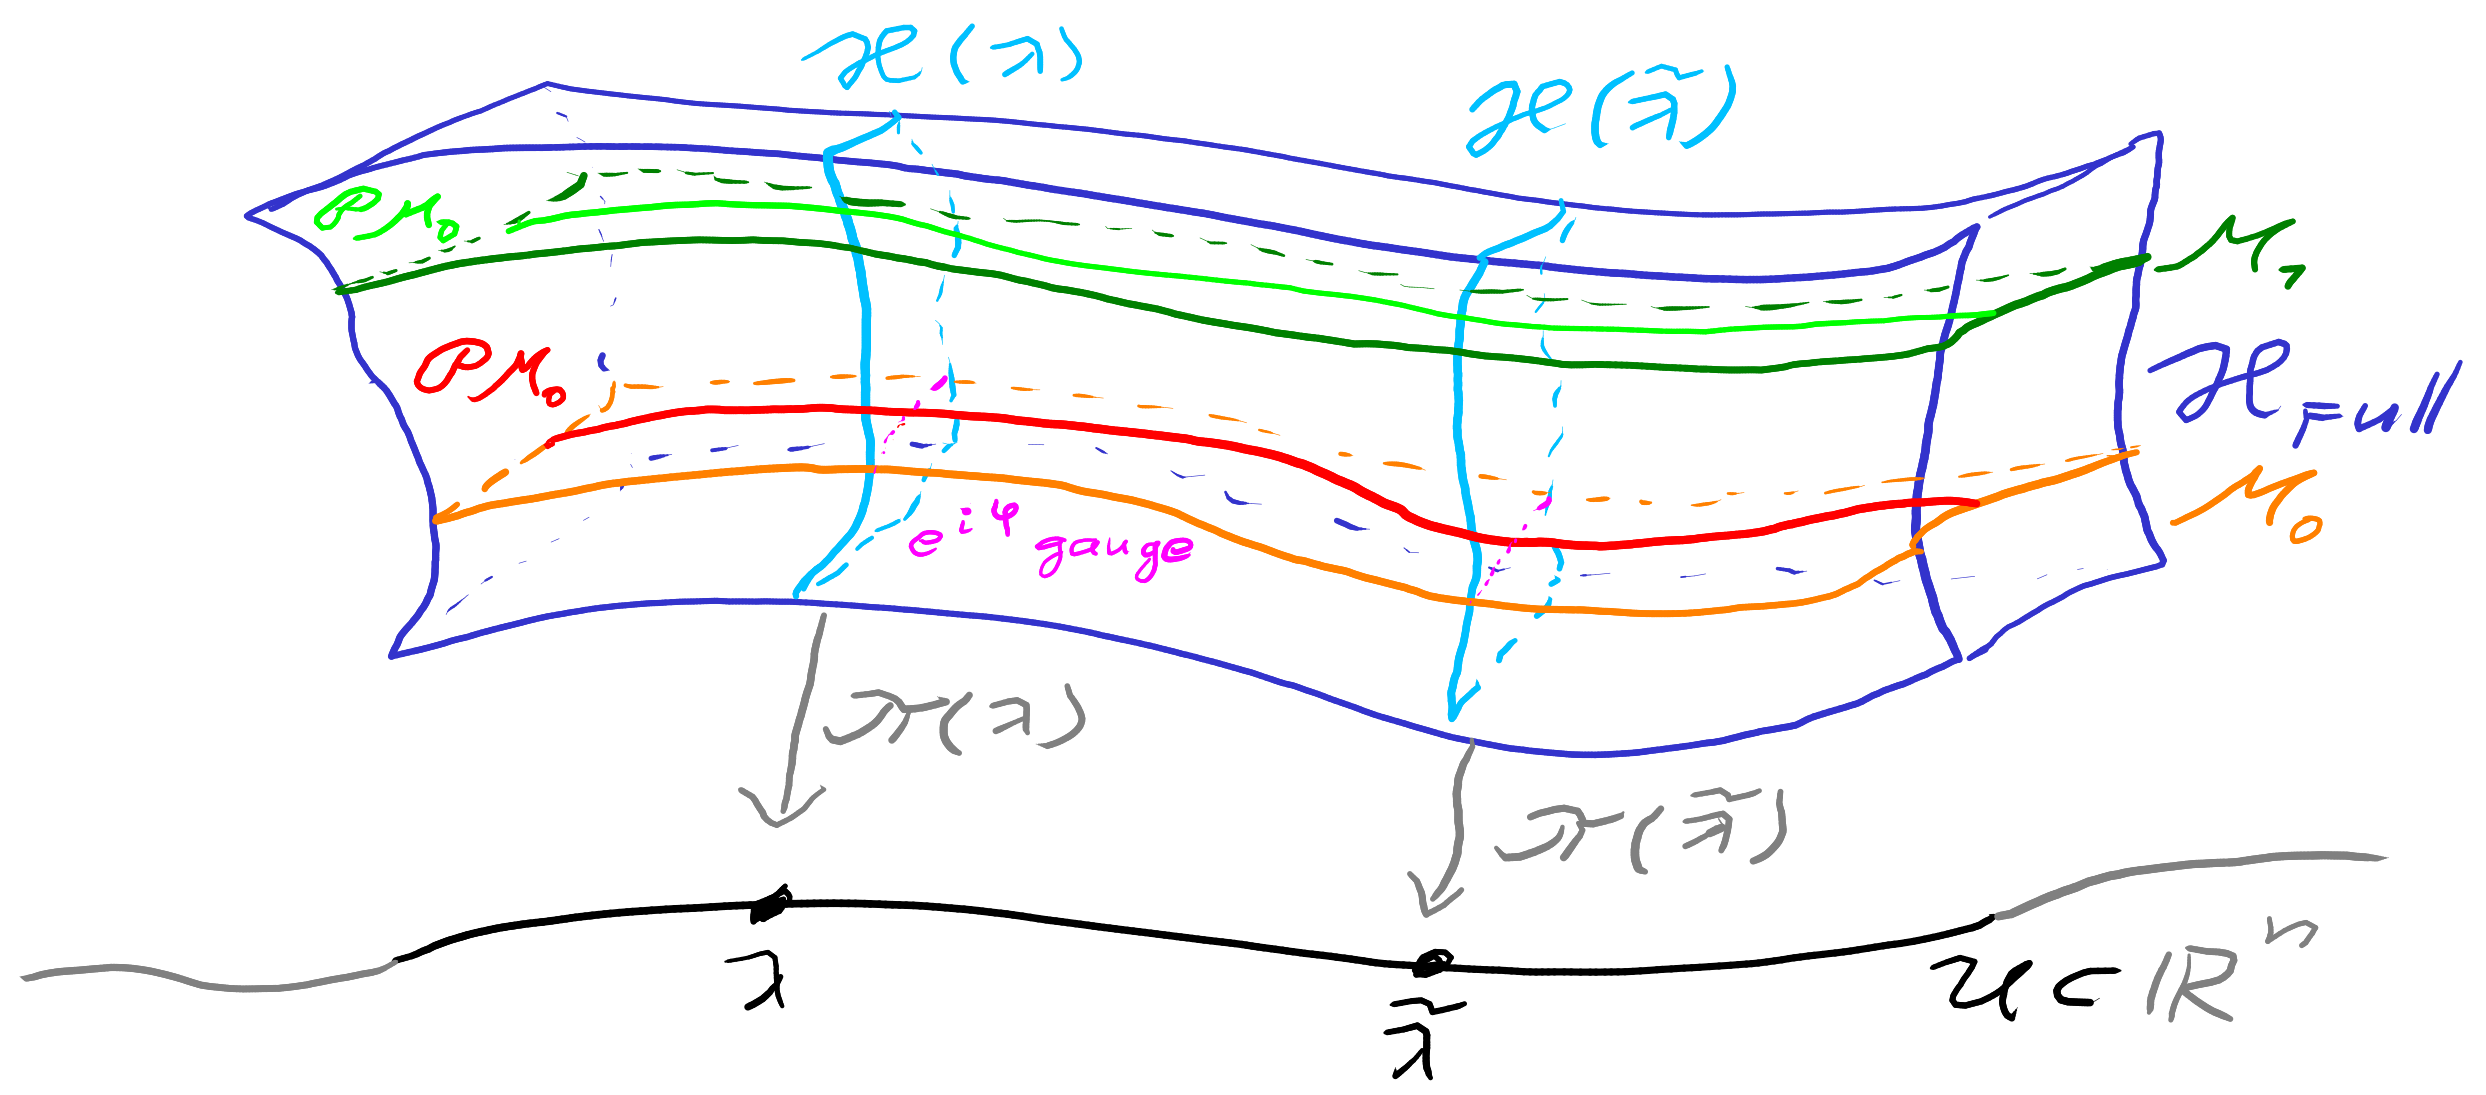
\includegraphics[width=\textwidth]{../img/manifold_full_1.png}
\caption{From the full Hilbert space we identified eigenstates. First was caused by the fiber structure and separates different Hilbert spaces $\HH(\llambda)$. Newly introduced sectioning correspond to eigenstates of individual Hamiltonians and creates Riemannian manifolds $\M_s$.}
    \label{fig:fullStructure}
\end{figure}






\section{Transporting states on state manifolds}
Let's now focus on decomposition of $\H_{full}$ to different state manifolds $\M_s$, as displayed on figure \ref{fig:manifoldCutIntuition}.

\begin{figure}[h]
    \centering
    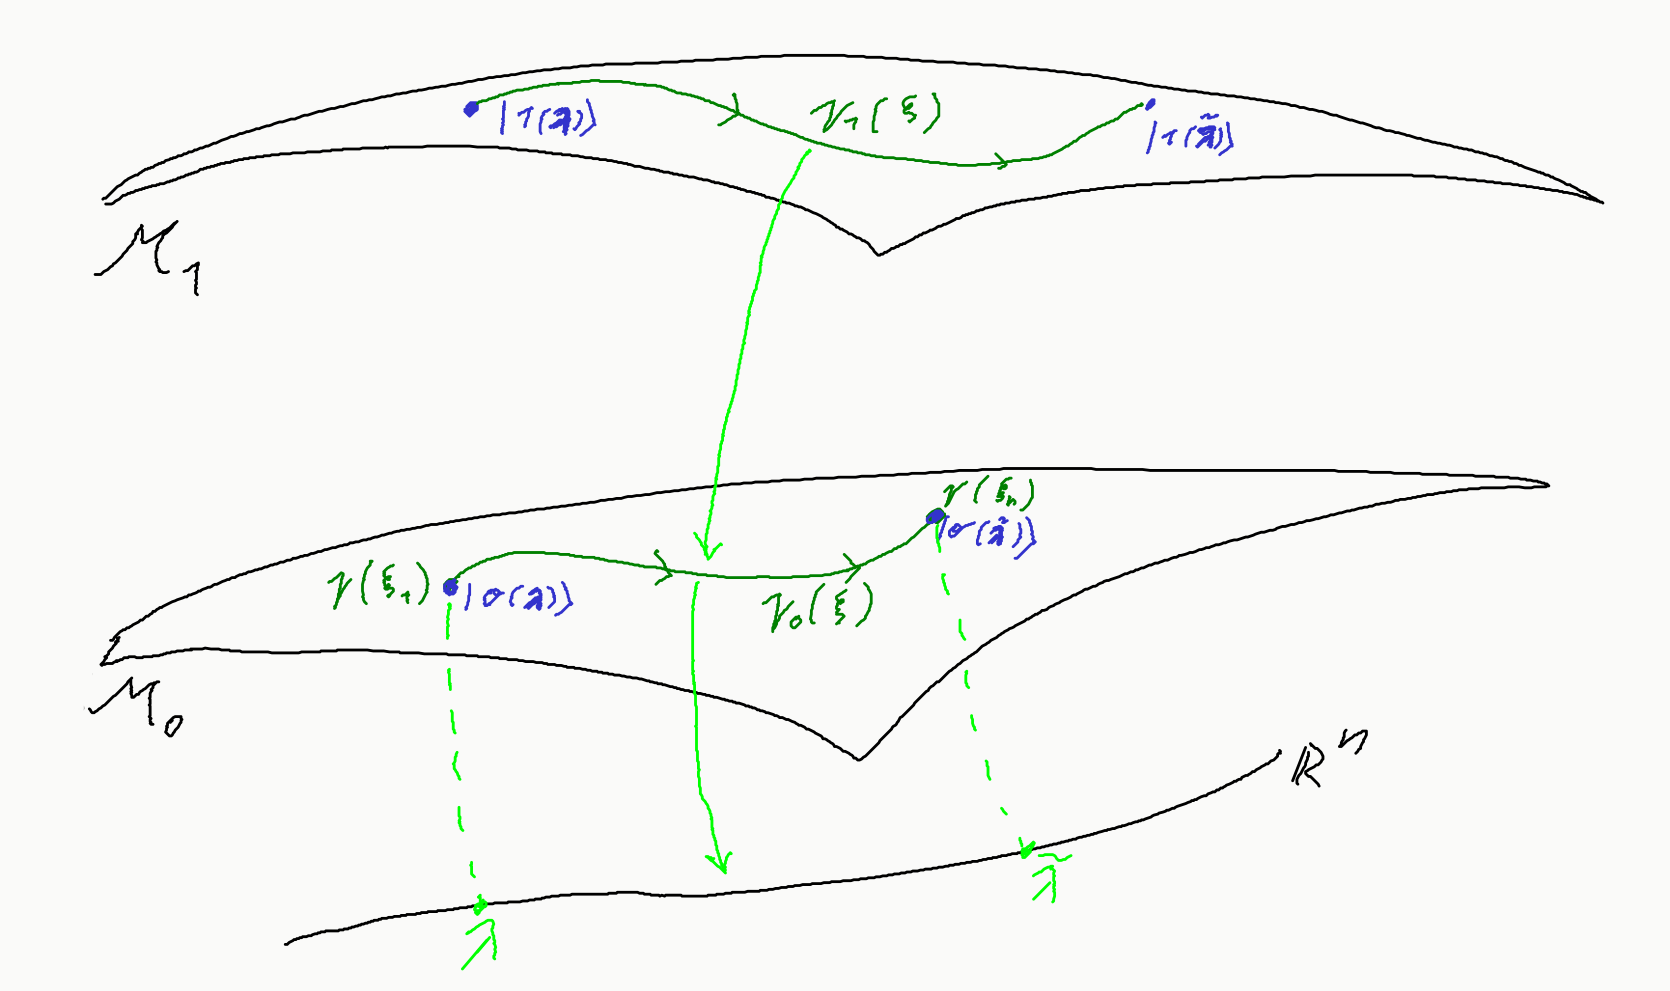
\includegraphics[width=\textwidth]{../img/manifoldCutIntuition.png}
\caption{Geometrical intuition to transport on fiber manifold sections $\M_s$.}
    \label{fig:manifoldCutIntuition}
\end{figure}

Changing the state from eigenstate $\ket{s(\llambda)}\in\M_s$ to $\ket{\psi(\tilde\llambda)}\in\M_s$ during some time period is unitary transformation and can be thought of as \emph{parallel transport on fiber bundle} between two states. Assuming the transport goes along curve parametrized by time $\gamma\coloneqq\{\llambda(t)|t\in(0,T)\}\subset \mathcal U$. The transported state can be written at any time as
\begin{equation}
    \kpsit = \Par_{\gamma_s(t)}\ket{s(\llambda(t))} = \exp\left(-i\int_0^tE_s(\tau)\d\tau)\right)\exp(i\gamma_s(t))\ket{s(\llambda(t))}.
    \label{eq:phasesOnManifold}
\end{equation}
Let's describe the meaning of two exponentials in this transport.
\subsubsection{Dynamical phase}
The first exponential in Eq. \ref{eq:phasesOnManifold}, the \emph{dynamical phase}, is well known solution to energy \Schrodinger equation \ref{eq:energySchrodinger} and depends only on time and energy spectrum during the transport. This dynamical phase changes the states only within the projective state manifold $\P\M_s$. 

\subsubsection{Geometrical phase}
The complication arises with the fact that our playground is a state manifold $\M_s$ and some element $e^{i\varphi}=e^{i\gamma_s(t)}$, called \emph{geometrical phase} needs to be included.\footnote{The usage of $\varphi$ as a geometrical phase is no coincidence, because it corresponds its to previous usage in gauge symmetry of quantum states.} This phase is generally non-integrable, meaning it depends on the whole path and cannot be written simply as $\gamma_s(\llambda)$. For some closed curve on
\begin{equation}
    C=\{\llambda(t)|t\in[0,T] \text{, such that }\llambda(0)=\llambda(T)\}\subset \mathcal U
\end{equation} 
we generally get $\Par_C \ket{\psi(\llambda)}\neq \ket{\psi(\llambda)}$. This property is sometimes more generally called an \emph{anholonomy} % and should be defined properly.
% \begin{definition}[Anholonomy]
%     Geometrical phenomenon, which causes some variable $V(\gamma(p))$ not to return to it's original value while varying it's parameter $p$ around some closed curve $\gamma(p)$. 
% \end{definition}
and geometric intuition can be seen on fig. \ref{fig:parallelTransportClosed}. 
\begin{figure}[h]
    \centering
    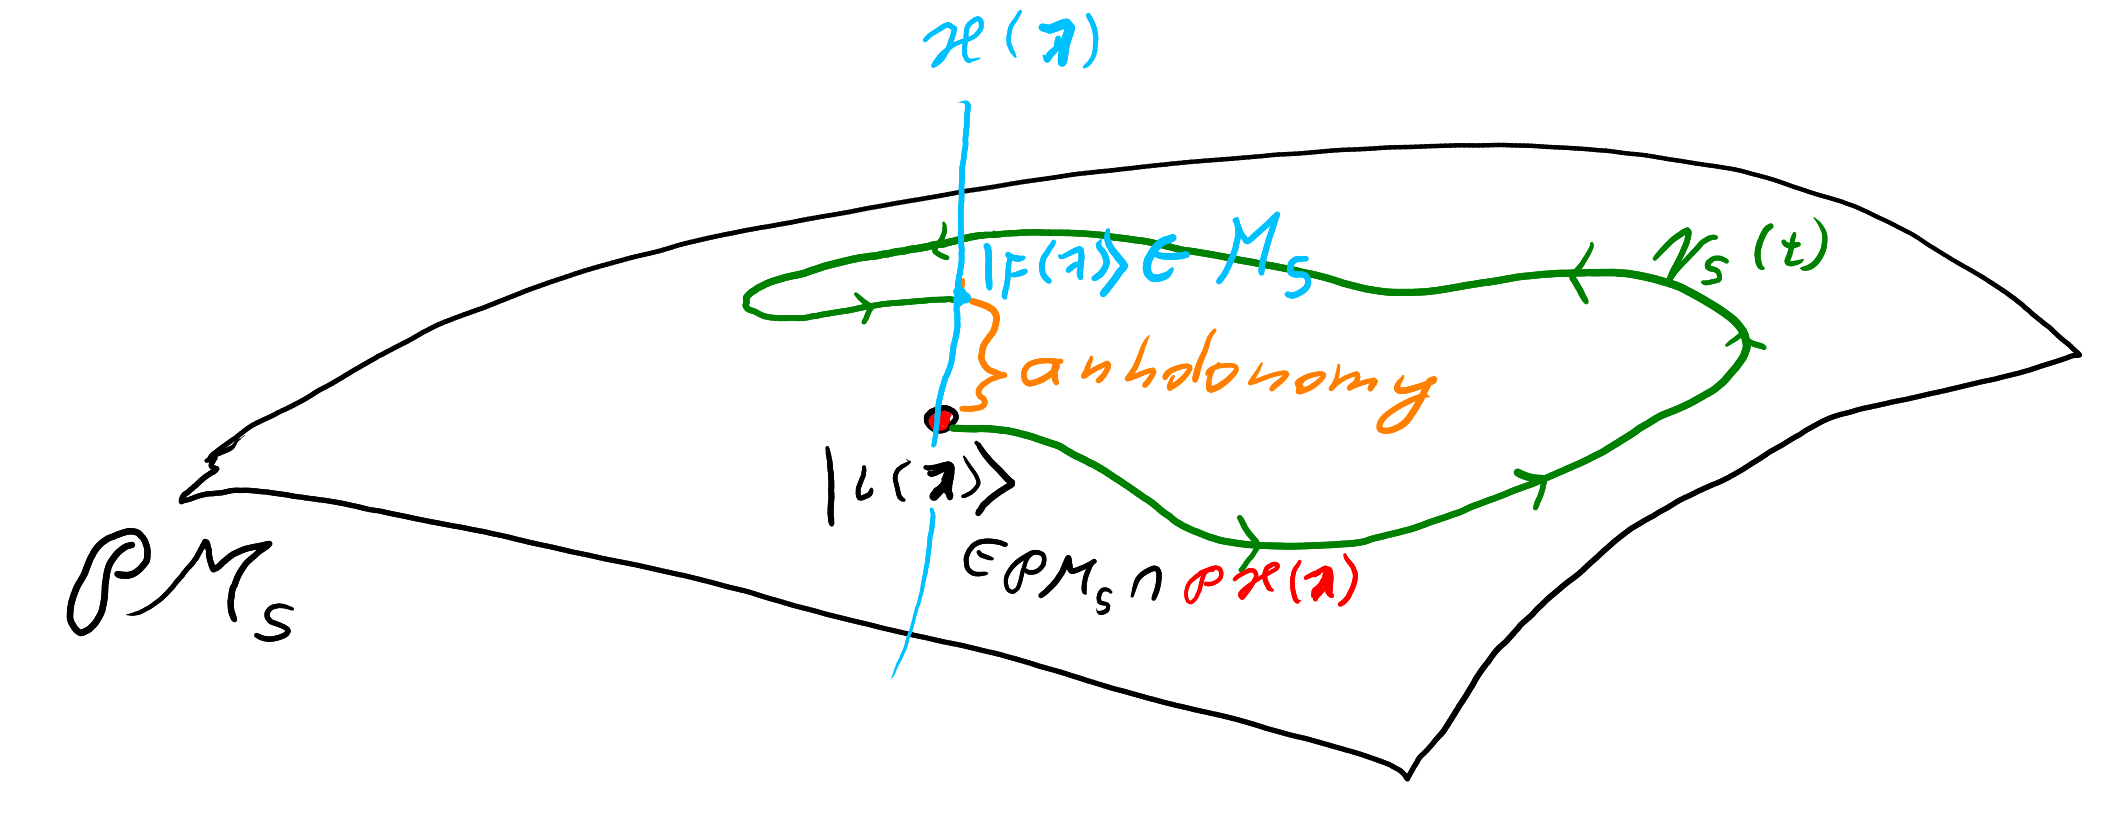
\includegraphics[width=0.8\textwidth]{../img/parallelTransportClosedCurve_1.png}
\caption{Parallel transport around some \greenn{closed curve $C$}. The \red{eigenstate} from $\P\M_s$ can be transported to another eigenstate in $\M_s$. The \reddd{anholonomy} represents their difference.}
    \label{fig:parallelTransportClosed}
\end{figure}

% For quantum states, the anholonomy can be measured as a non-zero angle between $\ket{V}$ and $\Par_C\ket{V}$, meaning
% \begin{equation}
%     \braket{V|\Par_C|V}\neq 0.
% \end{equation} 


Substituting general solution \ref{eq:phasesOnManifold} to Eq. \ref{eq:schrodinger} yields\footnote{Here the derivation along upper bound $F(x)\coloneqq\int_0^{g(x)}f(t)\d t \Rightarrow F'(x)=f(g(x))g'(x)$ for $f(t)\in L^1(0,g(x))$ and differentiable function $g$, is used.} 
\begin{align}
    \HH(\llambda(t))\kpsit &= i\der{}{t}\kpsit\\
    E_s(\llambda(t)) \ket{s(\llambda(t))} &= E_s(\llambda(t))\ket{s(\llambda(t))} -\der{\gamma(t)}{t}\ket{s(\llambda(t))}+ \der{}{t}\ket{s(\llambda(t))}\\
    \der{\gamma(t)}{t}&=i\braket{s(\llambda(t))|
    \der{}{t}|s(\llambda(t))}.
\end{align}
 Separating the dependence of vectors on driving parameter and time, we get
\begin{equation}
    \der{\gamma(\llambda(t))}{t} =i\braket{s(\llambda(t))|\partial_j s(\llambda)} \der{\llambda^j(\lambda)}{t} .
\end{equation}
Integrating this equation around some closed curve $C$ and assuming the dynamical phase to be zero, we get
\begin{equation}
    \gamma_s(C)=i\oint_C\braket{s(\llambda)|\partial_j s(\llambda)}\d \llambda^j.
    \label{eq:gammaCoint}
\end{equation}
We see, that the geometric phase does not depend on energy or time, only on the sequence of Hamiltonians, which means it depends only on the path itself.



\subsection{3-dimensional parametric space $\mathcal{U}$}
The problem of calculating Eq. \ref{eq:gammaCoint} lies in the element $\partial_\llambda s(\llambda)$, which locally requires knowledge of single-valued basis $\{\ket{0},\dots, \ket{n}\}$. This can be avoided in 3-dimensions using Stokes's theorem for $S$ as the surface with boundary $\partial S=C$, for coordinate gradient $\bm \nabla$
\begin{equation}
    \begin{split}
        \gamma_s(C) &= -\Im \iint_C \bm\d S \cdot \bm \nabla \times \braket{s(\llambda)|\bm \nabla n(\llambda)}\\
         &= -\Im \iint_C \bm\d S \cdot \braket{\bm \nabla s(\llambda)|\times|\bm \nabla s(\llambda)}\\
        &= -\Im \iint_C \bm\d S \cdot \sum_{m\neq s} \braket{\bm \nabla s(\llambda)|m(\llambda)}\times \braket{m(\llambda)|\bm \nabla s(\llambda)}\\
        &= -\iint_C \bm\d S \cdot \bm V_s(\llambda)
    \end{split}
    \label{eq:stokes}
\end{equation}
for 
\begin{equation}
    \bm V_s(\llambda) = \sum_{m\neq s} \Im \frac{
            \braket{s(\llambda)\bm \nabla_\llambda \HH(\llambda) |m(\llambda)}\times \braket{m(\llambda)|\bm \nabla_\llambda \HH(\llambda)|s(\llambda)}    
             }{
(E_m(\llambda)-E_s(\llambda))^2
             }.
\end{equation}
The element of summation $m=s$ in third step of derivation \ref{eq:stokes} is real, therefore has no influence on $\gamma_s$ and can be omitted. The last equivalence holds, because if we differentiate the \Schrodinger equation \ref{eq:energySchrodinger}, we get for any $\ket{s}\coloneqq \ket{s(\llambda)}\in \M_m,\;\ket{m}\coloneqq \ket{m(\llambda)}\in \M_m$
\begin{equation}
    \begin{split}
        \bm \nabla (\overbrace{\HH(\llambda)\ket{s}}^{E_s(\llambda)\ket{s}})&= (\bm\nabla \HH(\llambda))\ket{\bm \nabla s} +\HH(\llambda) \ket{\bm \nabla s}\\
        \braket{m|E_s(\llambda)|s}&= \braket{m|\bm \nabla \HH(\llambda)| s}+ \underbrace{\bra{m} \HH(\llambda)}_{\bra{m} E_m(\llambda)} |\bm\nabla s\rangle \\
        \braket{m|\bm \nabla s}&=
        \frac{\braket{m|\bm \nabla \HH(\llambda) |s}}
        { E_s(\llambda)-E_m(\llambda)}, \qquad s\neq m,
    \end{split}
\end{equation}

where we used $\ket{\bm \nabla s}\equiv\bm \nabla \ket{ s}$. 

Comparing the first expression in Eq. \ref{eq:stokes} with its last one and extending it to real numbers, we get
\begin{equation}
    \bm V_s(\llambda)=\bm \nabla\times\braket{s(\llambda)|\bm \nabla m(\llambda)}, 
    \label{eq:vectorPotentialDef}  
\end{equation}
defining \emph{vector potential} of $\bm V_s(\llambda)$. In addition, it extends our definition from single valued basis to any solution of \ref{eq:energySchrodinger}, thus instead of ground state manifold, we can use any $\M_s$.

As was mentioned, the above procedure from Eq. \ref{eq:gammaCoint} was performed only for three-dimensional space. Proper generalization to k-dimensional space would yield, see \citet{berry1984},
\begin{equation}
    \gamma_s(C) = -\iint_C (\bm\d S)^{\alpha\beta} \cdot\Im \frac{
            \overbrace{\braket{s(\llambda)\bm\d_\alpha \HH(\llambda) |m(\llambda)}}^{\in\TT_1\M}\wedge \overbrace{\braket{m(\llambda)|\bm\d_\beta\HH(\llambda)|s(\llambda)}}^{\in\TT_1\M}    
             }{
(E_m(\llambda)-E_s(\llambda))^2
             }.
\end{equation}






\section{Fidelity}
The \emph{fidelity} measures "closeness" of two quantum states. It is generally defined for two density operators $\hat\rho, \hat\sigma$ as
\begin{equation}
    \begin{split}
        \mathcal F&: \End(\H)\times \End(\H)\mapsto \C, \\
        &\mathcal F(\hat\rho,\hat\sigma)\coloneqq \left(\Tr \sqrt{\sqrt{\rho}\sigma\sqrt{\rho}}\right)^2.
    \end{split}
\end{equation}
For pure states $\hat\rho\eqqcolon\ket{\rho}\!\!\bra{\rho}$, $\hat\sigma\eqqcolon\ket{\sigma}\!\!\bra{\sigma}$, this reduces to
\begin{equation}
    \begin{split}    
        F&: \H\times\H\mapsto \C, \\
        &F(\ket{\rho},\ket{\sigma}) \equiv  \mathcal F(\hat\rho,\hat\sigma)\left| \braket{\rho|\sigma}\right|^2.
    \end{split}
\end{equation}



We can see it's physical meaning on the state manifolds, imagining \emph{quantum quench} (rapid change of some Hamiltonian parameters). In this case $F$ is the probability that system will remain in the new ground state and $1-F$ is the probability of exciting the system during this quench.






\section{\red{Metric and geometric tensor}}
As a playground for this chapter, we will choose the projective ground state manifold $\P\M_0\equiv \cup_{\llambda\in\R^d} \{\ket{o(\llambda)}\}$, but it can be easily generalized to any projective state manifold $\P\M_s$. This means the geometrical phase will be neglected, because the states are the physical states from the projective Hilbert space.
% Our first guess might be
% \begin{equation}
%     \d \tilde{s}^2 = \braket{i(\bm\llambda+\d\bm\llambda)|i(\bm\llambda+\d\bm\llambda)} = 1-2\Re{\braket{i(\bm\llambda+\bm\d\llambda)|i(\bm\llambda)}}.
% \end{equation}
% This is \emph{gauge dependent}, meaning that it depends on our choice of the wave phase, i.e. on observer. 

Let's first look at $\P\M_0$, which is needed to be \emph{gauge independent} in a sense, that the change in phase factor $\varphi$ of some state $\ket{o(\llambda)}\in \P\M_0\cap \H(\llambda)$ induces the change 
\begin{equation}
    \begin{split}        
        \ket{o(\llambda)}&\mapsto e^{i\varphi(\llambda)} \ket{o(\llambda)} \\
        &\,\Downarrow \\ 
        \braket{o(\llambda)|\bm \nabla o(\llambda)}&\mapsto \braket{o(\llambda)|\bm \nabla o(\llambda)} + i\bm \nabla \varphi(\llambda) 
    \end{split}
\end{equation} 
For $\varphi(\llambda)\in \mathcal C^2$ we see from Eq. \ref{eq:vectorPotentialDef}\red{to uz nevidim!!}, that gauge independent choice would be for infinitesimal change for example
\begin{equation}
    f=\braket{o(\bm\llambda+\delta\bm\llambda)|o(\bm\llambda)},
    \label{eq:fidelityDefinition}
\end{equation}
sometimes referred to as the \emph{fidelity amplitude of a ground state}. The meaning of fidelity as a probability transition between the states during some quench, leads to the definition of \emph{distance on $\M_0$}\footnote{$\d$ notation is in differential geometry assumed to be an exterior differential. On functions, it acts as $\d: \F\M\rightarrow \mathcal{T}_1\M$ and intuitively corresponds to total differential from functional analysis.}
\begin{equation}
    \d s^2 \equiv 1-F(\ket{o(\bm\llambda+\delta\bm\llambda)},\ket{o(\llambda)})= 1-\left|\braket{o(\bm\llambda+\delta\bm\llambda)|o(\bm\llambda)}\right|^2.
    \label{eq:distanceOnM0}
\end{equation}
We can easily check, that the axioms for metric distance holds:
\begin{itemize}
    \item identity of indiscernibles $s(\kpsi,e^{i\alpha}\kpsi) = 0 \Leftrightarrow \kpsi=\kphi$, $\alpha\in\R$,
    \item symmetry for any two states $\kpsi$, $\kphi$ is implied by $|\braket{\psi|\varphi}|=|\braket{\varphi|\psi}|$
    \item triangle inequality: $s(\kpsi,\ket{\psi_2}) <s(\kpsi,\kpsi_1) + s(\ket{\psi_1},\ket{\psi_2})$ for any $\ket{\psi_1}$.
\end{itemize}
From this, $g^\mu\nu$ is a metric tensor.

Because $1-f^2>0$, the first term of Taylor expansion is zero, thus we can use it for the metric tensor definition.

\begin{definition}[Metric tensor on projective state manifolds]
Because the projective state manifolds $\P\M_s$ are isomorphic to base manifold $\R^n$, we can define $g_{\mu\nu}: \R^n\times\R^n\rightarrow \R$ from
    \begin{equation}
        g_{jk}\d \bm \lambda^j \d\bm \lambda^k+\O(\lambda^3) \equiv \d s^2 = 1-\left|\braket{o(\bm\llambda+\delta\bm\llambda)|o(\bm\llambda)}\right|^2..
        \label{eq:metricTensorDef}
    \end{equation} 
   
\end{definition}
Let's decompose it to two parts with clear physical meaning.

This metric is called the \emph{Geometric tensor}, and can be expressed as 
\begin{equation}
    \chi_{\mu\nu}\coloneqq \braket{\partial_\mu o|\partial_\nu o}_c \equiv \braket{\partial_\mu o|\partial_\nu o} - \braket{\partial_\mu o|o}\braket{o|\partial_\nu o},
    \label{eq:geometricTensor}
\end{equation}
where shortened notation $\partial_\nu\coloneqq\pder{}{\lambda^\nu}$ was used. 

%taylor is wrong
% \begin{proof}[Proof for Geometric tensor expression] In one-dimensional case we get from eq. \ref{eq:fidelityDefinition} using Taylor expansion and shortened notation $o\coloneqq o(\lambda)$
%     \begin{equation}
%         f=1+\braket{\partial_\lambda o|o}\delta\lambda-\frac{1}{2}\braket{\partial_\lambda^2 o|o}\delta\lambda^2+\mathcal{O}(\lambda^3),
%     \end{equation}
%     which plugged into eq. \ref{eq:distanceOnM0} gives
%     \begin{equation}
%         \begin{split}
%             \d s^2&=1-\bar{f}f=\left[-\braket{o|\partial_\lambda o}\braket{\partial_\lambda o|o}+\frac{1}{2}\braket{\partial_\lambda^2 o|o}+\frac{1}{2}\braket{o|\partial_\lambda^2 o}\right]\delta \lambda^2.
%         \end{split}
%     \end{equation}
%     Generalizing for $\lambda\in \R^d$, we get\footnote{assuming Hermiticity of the derivative operator everywhere on the ground state manifold}
%     \begin{equation}
%         \d s^2=\left[-\braket{o|\partial_\mu o}\braket{\partial_\nu o|o}+\underbrace{\frac{1}{2}\braket{o|\partial_\mu \partial_\nu|o}+\frac{1}{2}\braket{o|\partial_\nu \partial_\mu| o}}_{\Re\braket{\partial_mu o|\partial_\nu o}}\right]\delta \lambda^\mu\delta \lambda^\nu.
%     \end{equation}
%     Because only symmetric part contributes in the sum in eq. \ref{eq:metricTensorDef}, this proves symmetric part of equation \ref{eq:geometricTensor} and shows, that some more general tensor (\emph{geometric tensor}) exists.
% \end{proof}

It is practical to decompose it to the geometric tensor
\begin{equation}
    \chi_{\mu\nu} \equiv g_{\mu\nu} - i\frac{1}{2} \nu_{\mu\nu},
\end{equation}
where the \emph{Fubini-Study tensor}\footnote{In some literature, this is called Geometric tensor}, as it's called, is metric on $\P\M_0$ and can be expressed as
\begin{equation}
    g_{\mu\nu} = \frac{\chi_{\mu\nu}+\chi_{\nu\mu}}{2} = \Re\braket{\partial_\mu o|\partial_\nu o}_c = \Re \sum_{o\neq j}\frac{\braket{o|\pder{\H}{\lambda^\mu}|j}\braket{j|\pder{\H}{\lambda^\nu}|o}}{(E_o-E_j)^2},
    \label{eq:metrictensorREdefinition}
\end{equation}
and the \emph{curvature tensor} a.k.a. \emph{Berry curvature} is
\begin{equation}
        \nu_{\mu\nu} = i(\chi_{\mu\nu}-\chi_{\nu\mu})= \Im\braket{o|[\curlyleftarrow{\partial}_\nu,\partial_\mu]|o}_c = -2 \Im \sum_{o\neq j}\frac{\braket{o|\pder{\H}{\lambda^\mu}|j}\braket{j|\pder{\H}{\lambda^\nu}|o}}{(E_o-E_j)^2},
    \label{eq:geom.tensorREdefinition}
\end{equation}
where $\curlyleftarrow{\partial}_\nu$ affects the covector on the left.


\subsection{Derivation of the geometric tensor}
\label{sec:derivationOfGeometricTensor}
To prove the correspondence of geometric tensor, described by eq. \ref{eq:geometricTensor}, to distance on $\M_0$, see eq. \ref{eq:distanceOnM0}, we start with eigenstate $\ket{o(\llambda)}\in \M_0\cap \H(\llambda)$. Changing parameters $\llambda$ to $\llambda+\delta \llambda$ results in Hamiltonian $\HH_f$ with eigenstates $\ket{s(\llambda+\delta \llambda)}\in \M_s\cap\H(\llambda+\delta \llambda)$, meaning it can be excited. Probability amplitude of going to such state is
\begin{equation}
    \begin{split}
        a_s&=\braket{s(\llambda+\delta\llambda)|o(\llambda)}\approx \delta\lambda^\mu\braket{\partial_\mu s(\llambda)|o(\llambda)} \\
        &= -\delta\lambda^\mu\braket{s(\llambda)|\partial_\mu|o(\llambda)}.
    \end{split}
\end{equation}

If we introduce the \emph{gauge potential}, aka \emph{calibration potential}, as\footnote{In SI units, the gauge potential is $\AA_\mu\equiv i\hbar\partial_{\mu}$}
\begin{equation}
    \AA_\mu\equiv i\partial_{\mu},
\end{equation}
the probability amplitude can be expressed as
\begin{equation}
   a=i\braket{s(\llambda)|\AA_\mu |o(\llambda)}\delta\lambda^\mu,
   \label{eq:probabilityOfTransitionIsGauge}
\end{equation}
which has meaning of matrix elements of the gauge potential. Probability of the excitation i.e. transition to any state $s>0$ from ground state is then (omitting the $\llambda$ dependence in notation)
\begin{equation}
    \begin{split}
        \sum_{s\neq 0}|a_s|^2&=  \sum_{s\neq 0} \delta \lambda^\mu \delta \lambda^\nu\braket{o|\AA_\mu|s}\braket{s|\AA_\nu|o}+\O(|\delta \lambda^3|) \\
        &= \delta \lambda^\mu \delta \lambda^\nu\braket{o|\AA_\mu \AA_\nu|o}_c\eqqcolon \delta \lambda^\mu \delta \lambda^\nu\chi_{\mu\nu}+\O(|\delta \lambda^3|),
    \end{split}
\end{equation}
where last term defines the geometric tensor.











\section{Berry phase and curvature}
Let's consider only the ground state manifold, because it will be used later on. Thought every step can be easily generalized to any state manifold $\M_s$.

On the ground state manifold $\M_0\equiv \cup_{\varphi\in\R}\cup_{\llambda\in\R^d} e^{i\varphi}\{\ket{o(\llambda)}\}$, the \emph{Berry connection} is defined as
\begin{equation}
    A_\mu(\llambda)\equiv \braket{o(\llambda)|\AA_\mu|o(\llambda)}\coloneqq -i\hbar \braket{o(\llambda)|\partial_\mu|o(\llambda)},
    \label{eq:berryConnection}
\end{equation}
which uses the decomposition of $\llambda$ to some basis, thus it empowers us to take derivatives in any direction in the base manifold $\R^d$ and thus the geometric tensor can be written as
\begin{equation}
    \chi_{\mu\nu}(\llambda) = \partial_\mu A_\nu(\llambda)-\partial_\nu A_\mu(\llambda)
\end{equation}
and the \emph{Berry phase}\footnote{
    The reasonability of this definition can be seen, if we assume the ground state of a free particle
        $\braket{\bm{x}|i(\llambda)}=i(\bm{x},\llambda)= |i(\bm{x})|e^{i\varphi(\llambda)}$,
    then the Berry connection is
    \begin{equation}
        A_\mu=-\int \d \bm{x}|i(\bm{x},\llambda)|^2\partial_\mu \varphi(\llambda) = -\partial_\mu \varphi(\llambda)
    \end{equation} 
    and Berry phase
    \begin{equation}
        \varphi_B=\oint_\mathcal{C} \partial_\mu \varphi \d \lambda^\mu,
    \end{equation}
    which represents total phase accumulated by the wave function. It is really the analogy for Berry phase in classical mechanics, which for example in the case Foucault pendulum on one trip around the Sun makes $\varphi_B=2\pi$
}
as the integral of the Berry connection along some closed curve $\mathcal{C}$
\begin{equation}
    \varphi_B\equiv-\oint_\mathcal{C} A_\mu(\llambda)\d \lambda^\mu=\int_\mathcal{S} \chi_{\mu\nu}(\llambda)\d \lambda^\mu \wedge \d\lambda^\nu,
\end{equation}
where we used the Stokes theorem for some area $\mathcal{S}$ with boundary $\partial\mathcal{S}=\mathcal{C}$.

Berry phase is usually zero, except for the cases, when the curve goes around some geometric tensor singularity, meaning $\mathrm{Ind}_a \gamma(\lambda)>0$. Those singularities appear in the system due to energy spectrum degeneracies, in the case of ground state manifold, when $E_1-E_0=0$. Those points are called \emph{diabolic}, because of their shape in the $(\lambda,\chi)$ parameter space.\footnote{https://en.wikipedia.org/wiki/Diabolo}












\section{General fidelity driving}

\subsection{APT}
From \cite{Rigolin2008}.
One important thing to bare in mind is \emph{locality of variables}. Let's call variable $V(s)$ \emph{\bluee{local}} if it depends only on infinitesimal sirrounding of $s$. These variables will be in shades of blue and non-local variables in shades of red.

The power series will be derived using a small parameter $v=1/T$. Starting again with
\begin{equation}
    \red{\ket{\Psi(s)}}=\sum_{p=0}^\infty v^p \red{\ket{\Psi^{(p)}(s)}},
    \label{eq:mainSeries}
\end{equation}

for 
\begin{equation}
    \red{\ket{\Psi^{(p)}(s)}}=\sum_{n=0} e^{-\frac{i}{v} \reddd{\omega_n(s)}}e^{i\reddd{\gamma_n(s)}}\redd{b_n^{(p)}(s)}\bluee{\ket{n(s)}}.
\end{equation}
Here the
\begin{align}
    \reddd{\omega_n(s)} &\coloneqq \frac{1}{\hbar}\int_0^s \bluee{E_n(s')}\d s'\\
    \reddd{\gamma_n(s)} &\coloneqq i\int_0^s \bluee{\braket{n(s')|\frac{\d}{\d s'}n(s')}}\d s' \equiv i\int_0^s \bluee{M_{nn}(s')}\d s'
    \label{eq:gammadef}
\end{align}
are so-called \redd{dynamical} resp. \redd{Berry (geometric) phase} and $\bluee{\ket{n(s)}}$ are solution to
\begin{equation}
    \bluee{\HH(s)\ket{n(s)}}=\bluee{E_n(s) \ket{n(s)}}.
\end{equation}
Variables $\reddd{\omega_n(s)}$ and $\reddd{\gamma_n(s)}$ are defined using integration over the whole protocol, therefore there are \emph{\red{non-local variables}}.
The problem now lies in determining $\redd{b_n^{(p)}(s)}$, which is also \red{nonlocal}. Because it depends on its relative \reddd{geometric} and \reddd{dynamical phase} to other \bluee{energy levels}, lets write it as a series
\begin{equation}
    \redd{b_n^{(p)}(s)}=\sum_{m=0} e^{\frac{i}{v}\reddd{\omega_{nm}(s)}}e^{-i\reddd{\gamma_{nm}(s)}}\blue{b_{nm}^{(p)}(s)},
\end{equation}
where $\reddd{\omega_{nm}} \coloneqq \reddd{\omega_m}-\reddd{\omega_n}$, $\reddd{\gamma_{nm}} \coloneqq \reddd{\gamma_m}-\reddd{\gamma_n}$.  The reason for \blue{locality} of $\blue{b_{nm}^{(p)}(s)}$ will be clear soon.

Inserting all to original series \ref{eq:mainSeries}, we get
\begin{equation}
    \red{\ket{\Psi(s)}}=\sum_{n,m=0}\sum_{p=0}^\infty v^p e^{-\frac{i}{v}\reddd{\omega_m(s)}}e^{i\reddd{\gamma_m(s)}}\redd{b_{nm}^{(p)}(s)}\bluee{\ket{n(s)}}.
    \label{eq:solve0}
\end{equation}

Because the initial state is eigenstate, we get initial conditions $\blue{b_{nm}^{(0)}(s)=0}$. In addition, one can rewrite equation \ref{eq:solve0} to the iteratively solvable form
\begin{equation}
    \frac{i}{\hbar}\bluee{\Delta_{nm}(s)}\blue{b_{nm}^{(p+1)}(s)}+\blue{\dot b_{nm}^{(p)}(s)}+\bluee{W_{nm}(s)} \blue{b_{nm}^{(p)}(s)}+\sum_{k=0,k\neq n}\bluee{M_{nk}(s)}\bluee{b_{km}^{(p)}(s)}=0,
    \label{eq:bSolution}
\end{equation}
for $\bluee{\Delta_nm(s)}\coloneqq \bluee{E_m-E_n}$, $\bluee{W_{nm}(s)}\coloneqq \bluee{M_{nn}(s)}-\bluee{M_{mm}(s)}$, where $\bluee{M_{mn}}$ is defined in Eq. \ref{eq:gammadef}. We can see that $\blue{b_{mn}^{(p)}}$, as a solution to Eq. \ref{eq:bSolution},\textbf{ only depends on difference between energy levels, eigenstates during the path and their directional derivatives. Not on the path itself}. All of those are easily obtained, once the driving path is prescribed.

    










\section{How to advantageously drive the system}

\subsection{Adiabatic driving}
Adiabatic transformation is such a transformation from $\M$ to $\M$, which does not excite the system, meaning the fidelity $f=1$. Generally it can be achieved by two ways -- infinitely slow transformation of states, or adding some \emph{counter-diabatic elements} to the Hamiltonian to counter the excitation.


In this chapter, we will be dealing with the system described by the finite-dimensional Hamiltonian $\HH(\llambda)$ which drives the system according to \Schrodinger equation from some initial state $\ket{s(\llambda}$ to $\ket{s(\tilde\llambda)}$ along the path $\gamma(\lambda)$. Before going throw the details of adiabatic transformations, let's define its meaning properly.

\begin{definition}[Adibaticity]
    Slow change of parameters driving Hamiltonian in a sense, that it does not excite the system and allows the system to return to the same energetic state after circulation around any closed path on the manifold with fidelity $f=1$.
\end{definition}


\subsubsection{Slow transports}
\citep{kolodrubez}[chap. 2.3]
As was mentioned in the introduction of this chapter, one way to change the system parameters without exciting it is to change the driving parameter slowly enough. The meaning of the word "slow" clears up next theorem.
\begin{thm}[Adiabatic theorem]
    \label{adiabaticTheorem}
    For Hamiltonian $\HH$ varying in the time range $T$, the solution of the Schrödinger equation 
    $$\HH(\lambda)\ket{\psi_n(\lambda)} = E_n(\lambda)\ket{\psi_n(\lambda)}$$
    with initial condition in x-representation $\braket{x|\psi(t=0}=\psi_n(x,0)$ can be approximated as
    \begin{equation}
      ||\psi(\lambda) - \psi_{ad}(\lambda)||\approx o\left(\frac{1}{T}\right)
    \end{equation}
    for \emph{adiabatic state}
    \begin{equation}
        \ket{\psi_{ad}}= e^{\theta_n(\lambda)}e^{\gamma_n(\lambda)}\ket{\psi(\lambda)},
    \end{equation}
    where we define \emph{nongeometrical phase} induced by energy transitions,
    $$\theta_n(\lambda)\equiv -\frac{1}{\hbar}\int_0^t E_n(\tau)\d \tau$$
    and \emph{geometrical phase}, also called \emph{Berry phase}
        $$\gamma_n(\lambda)\equiv \int_0^t \underbrace{i\braket{\psi_n(\tau)|\partial_t\psi_n(\tau)}}_{\nu_n(\tau)} \d \tau .$$
\end{thm}
\begin{myproof}
    \textcolor{blue}{TBD (is on wikipedia :)} )
\end{myproof}
Assume differentiable and non-singular Hamiltonian $\HH(\llambda)$ with degenerate basis $\{\ket{m,\llambda}\}_m$ called the \emph{adiabatic basis}. This is generally the family of adiabatically connected eigenstates\footnote{In the case of energy level crossing, the eigenstates are not unified, because transition between them is not adiabatical.} The transition amplitude between states for adiabatic change is
\begin{equation}
    0=\bra{m(\llambda)}\HH\ket{n(\tilde\llambda)} \quad \text{for }n\neq m, \forall \llambda,\forall \tilde \llambda.
\end{equation}
This can be driven along some curve $\gamma(\lambda)$, i.e. differentiated by $\partial_t$:
\begin{equation}
    \begin{split}
        0&=\bra{\partial_t m(\llambda)}\HH(\tilde \llambda)\ket{n(\tilde\llambda)}+ \bra{m(\llambda)}\overbrace{\partial_t\HH(\tilde \llambda)}^{\approx \partial_t\HH(\llambda)}\ket{n(\tilde\llambda)}+ \bra{m(\llambda)}\HH(\tilde \llambda)\ket{\partial_t n(\tilde \llambda)}\\
        &=E_n(\lambda)\braket{\partial_t m(\llambda)|n(\tilde \llambda)} + E_m(\lambda)\braket{m(\llambda)|\partial_t n(\tilde \llambda)}+ \bra{m(\llambda)}\partial_t \HH(\tilde\llambda)\ket{n(\tilde \llambda)}\\
        &= (E_m(\lambda)-E_n(\lambda))\underbrace{\braket{m|\partial_t (\tilde \llambda)}}_{-\frac{i}{\hbar}\bra{m}\AA_t\ket{n(\tilde \llambda)}} + \braket{m|\partial_t\HH|n(\tilde \llambda)}.
    \end{split}
\end{equation}

This can be rewritten in matrix form as
\begin{equation}
    i\hbar\partial_t\HH=[\AA_t,\HH]-i\hbar \hat{M}_t\qquad \text{for } \hat{M}_t\equiv -\sum_n\pder{E_n(\lambda)}{t}\ket{n(\lambda)}\bra{n(\lambda)}.
\end{equation}
$\hat{M}$ is diagonal in energetic basis and its elements has meaning of \emph{generalized force}. We can easily see that $[\HH,\hat{M}]=0$, implying
\begin{equation}
    [\HH,i\hbar\partial_t\HH-[\AA_t,\HH]]=0.
    \label{eq:komutation}
\end{equation}
This can be used as the definition for \emph{counter-diabatic potential} $\AA_t$, because it was obtained from only one assumption -- adiabaticity. The strength of this equation lies in fact, that it finds counter-diabatic potential without the need of Hamiltonian diagonalization.




\subsection{Counterdiabatic driving}
\subsubsection{Gauge potentials}
In section \ref{sec:derivationOfGeometricTensor} we introduced the gauge potential without proving its gauge meaning, but only stating its correspondence to transition probability, see eq. \ref{eq:probabilityOfTransitionIsGauge}.
\emph{Gauge transformations}, in classical mechanics called \emph{canonical}, can be defined such, that they \emph{preserve Lagrangian of the system under local transformations from some Lie group}. This implies, that gauge transformed Hamiltonian $\HH(\llambda)$ and $\HH(\llambda+\d \llambda)$ commutes with its canonically transformed version\footnote{This can be easily reformulated to the world of classical physics, where the commutator is replaced by Poisson bracket.} 
 \begin{equation}
     [\HH(\llambda),\HH(\llambda+\delta \llambda)]=0.
 \end{equation}

 To understand the meaning of gauge symmetries, let's first consider classical system and then move to quantum mechanics.




\subsubsection{Classical gauge potential}
In the Hamiltonian classical mechanics, we assume the manifold $\M$ as subset of the phase space defined by Hamiltonian $H=H(p_i,q_i)$, where momentum $p_i$ and position $q_i$ are assumed to form the orthogonal basis of the phase space
\begin{equation}
    \{q^i,p_j\}=\delta^i_j,
    \label{eq:canonicalCommutationDelta}
\end{equation}
which also defines \emph{calibrational freedom} in their choice. \emph{Canonical transformations} then by definition preserve this formula. Using the \emph{Poisson bracket}, defined as
\begin{equation}
    \{A,B\}\coloneqq \pder{A}{q^j}\pder{B}{p_j}-\pder{B}{q^j}\pder{A}{p_j},
\end{equation}
we will examine continuous canonical transformations generated by gauge potential $\A_\lambda$
\begin{align}
        q^j(\lambda+\delta\lambda)&=q^j(\lambda)-\pder{\A_\lambda(\bm{p},\bm{q})}{p_j}\delta\lambda \;\Rightarrow\; \pder{q^j}{\lambda}=-\pder{\A_\lambda}{p_j}=\{\A_\lambda,q^j\}
        \label{eq:gaugeAsGeneratorOfMotion1}\\
        p_j(\lambda+\delta\lambda)&=p_j(\lambda)-\pder{\A_\lambda(\bm{p},\bm{q})}{q^j}\delta\lambda \;\Rightarrow\; \pder{p_j}{\lambda}=-\pder{\A_\lambda}{q^j}=\{\A_\lambda,p_j\}.
        \label{eq:gaugeAsGeneratorOfMotion2}
\end{align}
Substituting this to relations of orthogonality \ref{eq:canonicalCommutationDelta}, we get
\begin{equation}
    \{q^j(\lambda+\delta\lambda),p_j(\lambda+\delta\lambda)\}=\delta^i_j + \mathcal{O}(\delta\lambda^2).
\end{equation}
 
If $\lambda$ is time parameter and $\A_t=-H$, equations \ref{eq:gaugeAsGeneratorOfMotion1},\ref{eq:gaugeAsGeneratorOfMotion2} are identical to the Hamilton equations
\begin{equation}
\begin{split}
    \dot{q}^j&=-\{H,q^j\} = \pder{H}{p_j}\\
    \dot{p}_j&=-\{H,p_j\} = -\pder{H}{q^j}.
\end{split}
\end{equation}
Because the Hamiltonian is generator of the movement in the phase space $(\bm{q},\bm{p})$, we can interpret $\A_t$ as the generators of the movement on $\M$. Other specific choice might be $\lambda=X^i$, which gives us the momentum components $\A_{X^i}=p_i$.

Generally every gauge symmetry is generated by its gauge potential and corresponds to some conserved property, as theorem of Emma Nöether states.





\subsubsection{Quantum gauge potential}
\citep{kolodrubez}[chap. 2.2]
The role of Poison brackets in quantum mechanics is taken by commutators, canonical transformations are called \emph{unitary transformations} and calibration freedom is hidden in the choice of basis. Now let's find some special basis transformations $\U$ between initial system $S$ and the transformed $\tilde{S}$. Both of them describe the system with Hamiltonian $\HH(\llambda)$ with eigenstates $\ket{n(\llambda)}$ and eigenstate manifolds $\M_n\equiv \cup_\llambda \{\ket{n(\llambda)}\}$. 

From fiber structure goes\footnote{especially from the fact, that all spaces $\HH(\llambda)$ are isomorphic to each other}, that any state of $\HH(\llambda)$ for $\forall \llambda\in U\subset \R^d$ can be decomposed as
    \begin{equation}
    \ket{\psi(\llambda)}\equiv \sum_n \psi_n(\llambda)\ket{n}
\end{equation}    
for some coordinate independent basis $\{\ket{n}\}_n$.
Then there exist unitary transformation
\begin{equation}
    \U(\llambda): \tilde S\rightarrow S,\quad \U(\llambda)\ket{m(\llambda)}=\ket{n}.
    \label{eq:transformationU}
\end{equation}
where scalar parameter $t$ is assumed to be changing along the path $\gamma(t)$, corresponding to situation on fig. \ref{fig:manifoldCutIntuition}. This satisfies
\begin{equation}
    i\hbar \partial_t \U(t)=\HH(t)\U(t)
    \label{eq:schrodingerForU}
\end{equation}
for $\HH$ the full Hamiltonian of the system and any point on $\tilde\gamma(t)$, along which the partial derivative is taken.


The wave function $\kpsi$ in $S$ can be decomposed using Schmidt decomposition\footnote{The Schmidt decomposition can be performed in finite dimension, or if the Hamiltonian is compact, which is not automatic in quantum mechanics. What's more, the Hamiltonian is usually not even bounded. Anyway, for simple systems with bounded energy we can assume so.}
\begin{equation}
    \ket{\psi(\llambda)} = \sum_{m,n}\psi_n(\llambda) \ket{m(\llambda)}\overbrace{\braket{m(\llambda)|n}}^{U_{mn}(\llambda)} =\sum_m \overbrace{\tilde{\psi}_m(\llambda)}^{\braket{m(\llambda)|\psi_n|n}}\ket{m(\llambda)},
\end{equation}
where $U_{mn}(\llambda)$ are matrix elements of unitary transformation $\U(\llambda)$. In this work, we will be interested only in the gauge transformations preserving energy of the system.





\subsubsection{Adiabatic gauge potential}

Adiabatic gauge potentials, sometimes just \emph{adiabatic potentials}, are generators of unitary transformations, so we can define them analogically to the classical case
\begin{equation}
    i\hbar\partial_\lambda \ket{\tilde{\psi}(\llambda)} = i\hbar \partial_\lambda\left(\U^+(\llambda)\ket{\psi} \right)= \underbrace{i\hbar\left(\partial_\lambda \U^+(\llambda)\right)\U(\llambda)}_{-\tilde{\AA_\lambda}}\ket{\tilde{\psi}(\llambda)}.
\end{equation}
The adiabatic potential $\tilde{\AA_\lambda}$ can be transformed to non-tilde system as
\begin{equation}
    \begin{split}
        \AA_\lambda&=\U(\llambda)\tilde{\AA_\lambda}\U^+(\llambda) = -i\hbar\U(\llambda)\big(\partial_\lambda \U^+(\llambda)\big) =\\
        &= -i\hbar\partial_\lambda\big(\underbrace{U^+(\llambda)U(\llambda)}_{\mathds{1}}\big)-\big(\partial_\lambda U(\llambda)\big)U^+(\llambda) \big) =i\hbar \big(\partial_\lambda U(\llambda\big)U^+(\llambda).
    \end{split}
\end{equation}
From this we get the equations for adiabatic potential in two systems
\begin{align}
    \AA_\lambda&=i\hbar \big(\partial_\lambda U(\llambda)\big)U^+(\llambda)
    \label{eq:adiabaticPotential}\\
    \tilde{\AA_\lambda} &= -i\hbar\left(\partial_\lambda \U^+(\llambda)\right)\U(\llambda)
    \label{eq:adiabaticPotentialTilde}
\end{align}
which can be shown to be Hermitian
\begin{equation}
     \tilde{\AA_\lambda}^+=i\hbar U(\llambda)^+\big(\partial_\lambda\U(\llambda)\big)=-i\hbar\big(\partial_\lambda\U(\llambda)^+\big)\U(\llambda) = \tilde{\AA_\lambda},
     \label{eq:counterdiabaticPotentialTwoSystems}
\end{equation}
analogically for non-tilde potential.
Using the eigenbasis of $\HH$, the matrix elements are
\begin{equation}
    \bra{n}\tilde{\AA_\lambda}\ket{m}=i\hbar\bra{n}\U(\llambda)^+\partial_\lambda\U(\llambda)\ket{m} = i\hbar\bra{n(\llambda)}\partial_\lambda\ket{m(\llambda)}.
\end{equation}
and because
\begin{equation}
    \bra{n(\llambda)}\AA_\lambda\ket{ m(\llambda)}= \bra{n}\tilde{\AA_\lambda}\ket{m},
\end{equation}
we get
\begin{equation}
    \AA_\lambda = i\hbar\partial_\lambda.
    \label{eq:adiabaticPotentialDefinition}
\end{equation}
% It's good to point out, that we were applying tilde operators to non-tilde states et vice versa. This can be justified only if we consider $\M$ big enough to contain all necessary states, which can be achieved during the transformation.



Adiabatic gauge transformations are  class of gauge transformations with fidelity $f=1$. This means, that if the system is driven by Hamiltonian $\HH(\llambda)$ with fidelity $f<1$, there exists such adiabatic potential $\A_\lambda$, that driving of the same system using $\HH-\A_\lambda$ has fidelity $f=1$.

The adiabatic gauge potentials can then be understood as affine connections defining the parallel transport on fiber bundle, if we define covariant derivative as
\begin{equation}
    D_\mu=\partial_\mu+i\AA_\mu,
\end{equation}
which yields $D_\mu\ket{\psi_n}=0$ for every eigenstate, which yields, that the transport of eigenvalues on $\M_0$ is parallel. $\AA_\mu$ is generally defined \ref{eq:adiabaticPotential}, which generally gives non-zero covariant derivative for states not belonging to $\M_0$. 

Finding of those potentials has many practical applications, so let's introduce one analytical procedure of finding them.






\subsubsection{Performing counter-diabatic driving}
\citep{kolodrubez}[page 15--17] The main idea of a counter-diabatic driving is, that any excitation of the system can be countered by adding so called \emph{counter-diabatic potential} to the Hamiltonian. Consider again any eigenstate $\kpsit$ of the Hamiltonian $\HH=\HH(\lambda)$ driven along the curve $\gamma(\lambda(t))$ on $\M_0$ depending on time $t$, during which the fidelity $f\neq 0$. Because the system is not measured during the trip, it can't be stated if or if not it was excited, but the main goal here is to make fidelity zero, which is iff $\tilde H$ is diagonal. For diagonalizable Hamiltonian, there exist a transformation, see eq. \ref{eq:transformationU}, for which the fidelity will be zero. Such a transformation does not have to be unique, but we can choose any one of them. This can be seen more clearly from direct transformation of the Schrödinger equation. 

The Schrödinger equation
\begin{equation}
    i\hbar \der{}{t}\ket{\psi(\lambda)} = \HH(\lambda)\ket{\psi(\lambda)}
\end{equation}
can be transformed using 
\begin{equation}
    \U(\lambda)^+  \ket{\psi(\lambda)} = \ket{\tilde\psi(\tilde\llambda)},
    \label{eq:transformationUtimeDependentH}
\end{equation}
for which $\tilde H \coloneqq\U^+\HH\U$ is diagonal, leading to
\begin{align}
    i\hbar \der{}{t}(\U(\tilde\llambda)\ket{\tilde \psi(\tilde\llambda)}) &= \HH(\lambda)\U(\tilde\llambda)\ket{\tilde \psi(\tilde\llambda)} \\
    i\hbar \der{\lambda}{t}\partial_\lambda\U(\tilde\llambda)\ket{\tilde \psi(\tilde\llambda)} + i\hbar \U(\tilde\llambda)\der{}{t}\ket{\tilde \psi(\tilde\llambda)} &= \HH(\lambda)\U(\tilde\llambda)\ket{\tilde \psi(\tilde\llambda)}.
\end{align}

This can be rewritten using adiabatic potential from eq. \ref{eq:adiabaticPotentialDefinition}, using \emph{dot} notation for time derivatives and omitting the points in which the objects are evaluated, as
\begin{equation}
    i\hbar \der{}{t}\ket{\tilde\psi} = \left[\U^+\HH\U-\dot{\lambda}\tilde{\AA_\lambda}\right]\ket{\tilde\psi} = \left[\tilde H-\dot{\lambda}\tilde{\AA_\lambda}\right]\ket{\tilde{\psi}} \eqqcolon \tilde{H}_m \ket{\tilde{\psi}},
\end{equation}
where the term $-\dot{\lambda}\tilde{\AA_\lambda}$ is called \emph{Galilean} and $ \tilde{H}_m$ is the Hamiltonian in transformed system. Because $\tilde{H}$ is diagonal, it drives $\ket{\tilde{\psi}}$ with fidelity $f=1$. This means that for any driving defined by $\HH(\lambda(t))$, which defines the unitary transformation $\U$, there exists such \emph{counter-diabatic potential} $\AA_\lambda$, that $\HH_m + \dot{\lambda}\AA_\lambda$ has $f=1$.


% Intuition for transformations using original Hamiltonian vs. transformed one can be seen on fig. \ref{fig:counterdiabaticPotential}. It is good to point out, that the eigenstates on this figure belong to the space $\P\M$, but the paths itself need to be considered in the whole $\M$, which can be seen as the phase change described by equation \ref{eq:evolutionUduringTransition}.

% \begin{figure}[h]
%     \centering
%     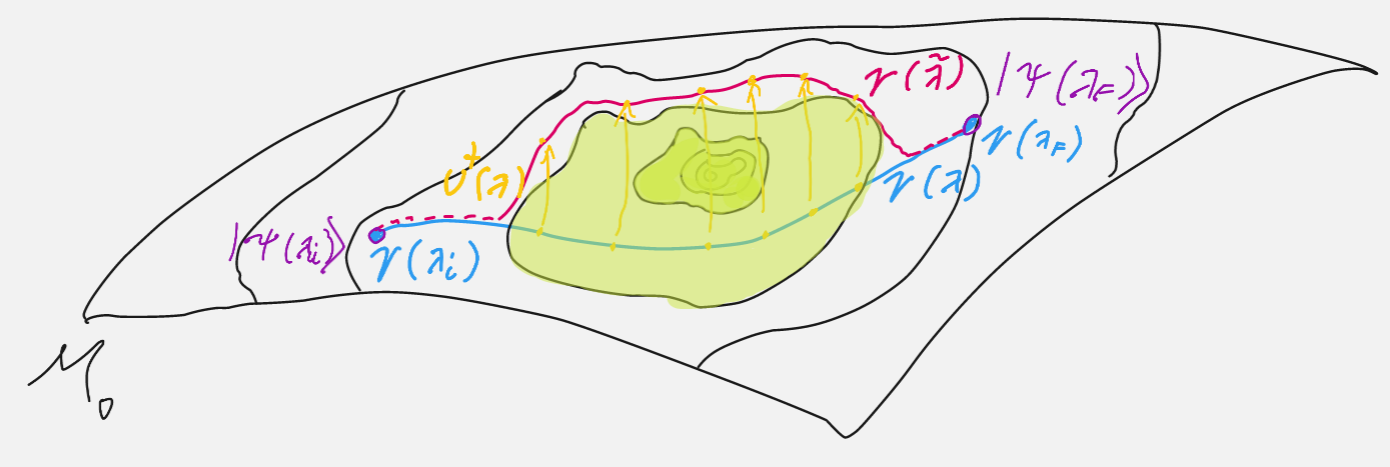
\includegraphics[width=\textwidth]{../img/counterdiabaticPotential.png}
%     \caption{Comparison between transport by Hamiltonian $\HH$ (blue path $\gamma(\lambda)$ and the one with counter-diabatic potential added (pink path $\gamma(\tilde\lambda)$), which has zero fidelity. The nonzero fidelity area for path $\gamma(\lambda)$ is marked green and initial and final states $\ket{\psi(\lambda_i)}$, resp. $\ket{\psi(\lambda_f)}$ are marked purple.}
%     \label{fig:counterdiabaticPotential}
% \end{figure}
This procedure does not directly tell us how to calculate the counter-diabatic potential, only states its existence. For many simple cases the calculation can be done analytically, but most often some approximation methods are needed.


\begin{figure}[h]
    \centering
    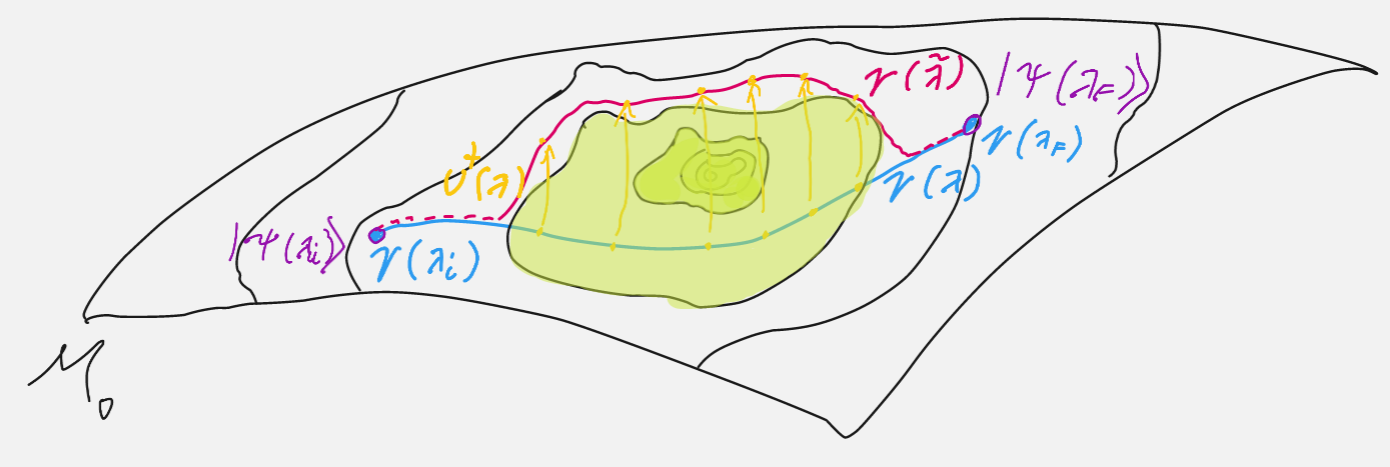
\includegraphics[width=\textwidth]{../img/counterdiabaticPotential.png}
\end{figure}




\subsubsection{Explicit form}
If we now consider the parametrization with time $t\coloneqq t$, $\U$ can be explicitly expressed according to \textcolor{red}{ansatz} in eq. \ref{eq:phasesOnManifold} as
\begin{equation}
    \U(t)=\sum_n \exp\left(\frac{i}{\hbar}E_n(\tau)\d \tau - \int_0^t \braket{s(\tau)|\partial_\tau n(\tau)}\d\tau\right)\ket{s(t)}\bra{s(0)}.
    \label{eq:evolutionUduringTransition}
\end{equation}
Inserting to eq. \ref{eq:schrodingerForU}, we get explicit form of the Hamiltonian, which can be decomposed into the diagonal form of the original Hamiltonian and a counter-diabatic potential
\begin{equation}
    \HH(t)=\sum_n \ket{n}E_n\bra{n}+ i\hbar \sum_n\ket{\partial_\lambda n}\bra{n}-\braket{n|\partial_\lambda n}\ket{n}\bra{n}\eqqcolon \HH_0(t)+\HH_1(t),
\end{equation}
for shortened notation $\ket{n}\equiv \ket{n(t)}$, analogically for bras. Using
\begin{equation}
    \HH_0(t)\ket{n}=E_n\ket{n}\quad \Rightarrow\quad \braket{m|\partial_\lambda n}=\frac{\braket{m|\partial_\lambda\HH_0| n}}{E_n-E_m}
\end{equation}
we have explicit formula
\begin{equation}
    \HH_1(t)= i\hbar \sum_{m\neq n}\frac{\ket{m}\braket{m|\partial_\lambda\HH_0| n}\bra{n}}{E_n-E_m}
    \label{eq:explicitCounterDiabaticPotential}
\end{equation}











% \section{\textcolor{blue}{Approximations of adiabatic potentials}}
% Adiabatic potentials can be calculated from the principal of minimal action, which leads to variational method.

% If the difference between eigenstates of $\HH$ is small, or generalized force between some states is zero, the computation of the adiabatic potential is numerically unstable. The knowledge of exact adiabatic potential would allow to maintain the system in the ground state thus not exciting it, as the Eigenstate thermalization hypotheses states.

% \begin{hypot}[Eigenstate thermalization hypotheses]
%   For the difference between eigenstates of $\HH$ and extensive thermodynamic entropy $S$, it holds that
%     \begin{equation}
%     E_n-E_m\propto \exp\left(\frac{S}{2}\right).
%   \end{equation}
%   If the states are close, better approximation would be $E_n-E_m\propto \exp(S)$. For matrix elements it holds, that they vanish exponentially with the characteristic scale of the system $a$, i.e.
%   \begin{equation}
%     \bra{m}\AA_\lambda\ket{n} = i\hbar\frac{\braket{m|\partial_\lambda \HH|n}}{E_m-E_n} \propto \exp(-a).
%     \label{eq:thermalizationMatrixElements}
% \end{equation}
% \end{hypot}
% Fortunately in the limit "number of particles" $\rightarrow \infty$ the expression in eq. \ref{eq:thermalizationMatrixElements} converges.



% \subsection{Variational methods}
% In the case of simple systems, the adiabatic potentials can be found analytically, but for more complicated Hamiltonians we will be forced to use approximations, or some perturbational and variational methods.